\chapter{Multiple Drift Detector} \label{chapt:MDD}

In this chapter we introduce multiple drift detector (MDD), a framework for human in the loop detection of multiple types of drift. Section \ref{mdd:motivation} discusses the motivation for MDD. Section \ref{mdd:algorithm} provides the algorithms pertaining to MDD. Section \ref{mdd:graphics} introduces a graphical interface for MDD. Section \ref{mdd:illustration} illustrates the utility of MDD within the medical referrals triage motivating example. Section \ref{mdd:conclusion} summarises this chapter and discusses future work.

%-------------------------------------------------------------------
% MOTIVATION
%-------------------------------------------------------------------

\section{Motivation} \label{mdd:motivation}

There is a standard ``grammar" of concept drift detection methods, in which the problem is formulated according to certain axioms. The import of these axioms varies significantly. Some are universal, others only common. Some are implicit, others explicit. Some are fundamental, others incidental and easily worked around. Some have important consequences, others are trivial. If the axioms do not obtain, then this will limit the applicability of the drift detection method. Below are some axioms we have identified, which are likely to deviate from the reality of practical applications, with discussion of how often they are adhered to:
\begin{itemize}
  \item {\bf Stable instance distribution} - Degradation in model accuracy may occur because 1) the model has gotten worse at predicting labels for specific instances, or 2) the proportion of instances which the model is bad at predicting has increased. Retraining will not necessarily be helpful in the second case, as there may be irreducible error. However, to our knowledge there are no extant concept drift detection methods which account for the possibility of changes in the instance distribution, and try to differentiate the two sources of increased error.
  \item {\bf Immediate labelling} - Labels become available immediately after the model has made its prediction. To our knowledge, there is no work on concept drift which entertains the possibility that this is not the case.
  \item {\bf Indexed time} - Instances arrive at regular time intervals, or periodic batches. % To our knowledge, there is no work on concept drift detection which accounts for instances arriving at irregular intervals.
  \item {\bf No human-in-the-loop} - A human is neither available nor necessary to assist in the model retraining process. To our knowledge, there is no work on human-in-the-loop concept drift detection or adaptation.
  \item {\bf Non-interpretability} - It is not necessary to understand {\it how} the joint feature-label distribution is changing, only to know that it {\it is} changing. Drift detection methods vary in interpretable they render the evolution of a data stream. DDM provides almost no additional information beyond its verdict on whether concept drift has occurred, whereas ADWIN provides p-values for all possible drift points, as well as estimates of the error rates before and after the drift point. %However, none have explicitly held interpretability as a goal.
  \item {\bf Binary labels} - All instances are classified into the positive and negative class.
  \item {\bf Balanced class labels} - Prior to DDM-OCI, concept drift detection work had tended to implicitly assume that labels would be balanced. Since DDM-OCI, LFR and PerfSim have explicitly accounted for labels being potentially unbalanced.
  \item {\bf Efficiency over accuracy} - Concept drift detection is often discussed in the context of data streams, in which computational resources are at a premium due to a high throughput of instances. Some drift detection methods embrace this axiom, such as SEED which uses reservoir sampling. However, there are also detection methods which sacrifice efficiency for accuracy, such as ADWIN.
  \item {\bf Online learning} - To our knowledge, all investigations into concept drift have expected the model to be learning online from new instances as they arise. The possibility of a model being trained and frozen ahead of the data stream on historical instances has not been explored. However, for most drift detection methods this makes no practical difference, so this is not a real impediment.
\end{itemize}

In practical data science, any of these axioms may be violated. As an illustration, we return to our motivating example of  GP referrals triage, and see whether the axioms obtain:
\begin{itemize}
  \item {\bf Stable instance distribution} - The instance distribution is likely to change due to changes in demographic, epidemiological, or other factors. Thus this axiom does not hold.
  \item {\bf Immediate labelling} - There may be a considerable delay between a referral document arriving and it being labelled by a clinician. Arbitrarily many new documents could arrive in this interval.
  \item {\bf Indexed time} - Referrals and labels will arrive at irregular intervals, and will display changes in frequency over time.
  \item {\bf No human-in-the-loop} - Because retraining the model requires coordination by a consulted data scientist, a human is both necessary and available for model retraining.
  \item {\bf Non-interpretability} - Interpretability is crucial so that clinicians and data scientists can make informed decisions about what actions to take after concept drift has been detected.
  \item {\bf Binary labels} - Four priority levels are used to categorically label referral documents.
  \item {\bf Balanced class labels} - Medium-priority labels (2 and 3) are more common than extreme priority labels (1 and 4).
  \item {\bf Efficiency over accuracy} - The throughput of instances is fairly low, on the order of one referral document per hour. A powerful GPU machine is detected to modelling the referral data, so computational resources are available for comprehensive drift detection methods. Furthermore, given the high-stakes nature of medical triage, it is essential to make use of these resources to detect concept drift as precisely as possible.
  \item {\bf Online learning} - The model is pre-trained on historical referral data and frozen prior to deployment on the data stream.
\end{itemize}

This illustrates that existing approaches to concept drift are not necessarily appropriate for practical data science, at least without modification. And in particular, existing methods are certainly not appropriate for our motivating example of GP referrals triage. In the next section, we consider operationalisations of concept drift which will be better suited for practical data science.

\subsection{Operationalisations of Concept Drift} \label{Background:operationalisations}
% NOTE: I intend to move this to Chapter 2, but I include it here because it sets up the next section.

Concept drift is a change in the instance-label joint distribution. That is, concept drift is the event
\begin{equation}
  D(x,y)
\end{equation}
where $D(z)$ denotes a change in the distribution of $z$. Attacking this problem directly is frequently too hard to be directly tractable. The most direct approach would be to apply multidimensional change-point detection methods to the joint distribution. In domains with high-dimensional feature space and complex, non-linear relationships between features and labels, these methods will be infeasible. In general, detecting a change in the joint distribution is strictly harder than modelling the relationship between labels and features to begin with. So the techniques used for change point detection should be at least as sophisticated as those used in modelling the data.

Most drift detection methods therefore operationalise the concept drift detection task. Rather than directly detecting a change in the joint distribution, they instead detect an {\it increase in the error rate}. Under a stable joint distribution, model accuracy should either remain steady, or decrease if the model is learning. We denote this operationalisation as
\begin{equation}
  D(x,y) \Leftarrow D_-(y=\hat{y})
\end{equation}
where $D_-(z)$ indicates a decrease in $\mathds{E}[z]$, and $\Leftarrow$ means ``is operationalised as". We call this the {\bf accuracy operationalisation}. It appears to have been introduced by Widmer and Kubat, and has since been employed in the majority of drift detection methods.

Klinkenberg and Renz expanded on the above operationalisation, and monitor each of accuracy, precision of the positive class, and recall of the positive class for decreases. This can be expressed
\begin{equation}
  D(x,y) \Leftarrow D_-(y=\hat{y}) \vee  D_-(y=1|\hat{y}=1) \vee D_-(\hat{y}=1|y=1)
\end{equation}
where the conjuncts indicate accuracy, precision, and recall, respectively.

Wang et al. argue that if a data stream contains imbalanced classes, then a degradation in the model's ability to predict the minority class will be difficult to detect under the accuracy operationalisation. They propose operationalising concept drift as a) detecting class imbalance, and b) detecting a drop in the recall of the minority class. That is
\begin{equation}
  D(x,y) \Leftarrow D(y) \vee D_-(\hat{y}=m|y=m)
\end{equation}
where $m$ is the minority class.

Wang\footnote{Not the same Wang.} and Abraham note that there are some deleterious changes in a model's confusion matrix which previous operationalisations will fail to detect. For comprehensiveness, they propose monitoring both precision and recall for both classes:
\begin{equation}
  D(x,y) \Leftarrow D_-(y=\hat{y}|y) \vee D_-(y=\hat{y}|\hat{y}).
\end{equation}
We will call this the {\bf precision-recall operationalisation}.

\subsection{Practical Operationalisation}

As mentioned in Section \ref{Background:operationalisations}, there are several operationalisations of concept drift which have been proposed. Which of these is most appropriate for practical data science applications? To answer this, we should consider what our objective is in concept drift detection. Upon detecting concept drift, there are three actions we might want to take
\begin{enumerate}
  \item retrain the model using a (recent) subset of the data if it is no longer fit for purpose, or
  \item recall the model if it is no longer fit-for-purpose and cannot be made so by retraining, or
  \item leave the model as-is if it is still fit-for-purpose despite the concept drift.
\end{enumerate}
In our motivating example of GP referrals triage, each of these could be manifested as:
\begin{enumerate}
  \item The triage decision making process has changed, so the model should be retrained on data since that change.
  \item The model is required to have an accuracy of at least 98\% to be ``clinically safe", but due to irreducible error the accuracy is stuck at 95\%. The model should therefore be recalled.
  \item The model has deteriorated slightly in its ability to distinguish between priority 1 and priority 2 referrals. But because there is little practical consequence in confusing these (the important thing is to accurately classify priority 3 and priority 4 labels), it is decided that the model should remain as-is.
\end{enumerate}
Which of these actions is appropriate will depend on the kind of concept drift which has occurred.
\begin{itemize}
  \item {\bf On-manifold feature drift} If the distribution of instances changes such that some kinds of instances become more prevalent and others less prevalent, but the manifold on which instances exist stays the same, then model performance metrics may degrade, however this may be due to changes in irreducible error, and retraining will probably not be necessary. However, if the performance degrades sufficiently, it may be necessary to recall the model.
  \item {\bf Off-manifold feature drift} If the distribution of instances changes such that new instances are occurring which were not part of the original manifold, then the model will not be able to predict the correct label for these instances and will require retraining.
  \item {\bf Real drift} If the relationship between instances and labels changes, then the model will require retraining.
  \item {\bf Label drift} may indicate that a model requires recall. In the GP referrals triage example, if the model starts predicting the same priority for {\it all} referrals, then it will not be fit-for-purpose.
\end{itemize}
Note that feature and label drift may be detected earlier than real drift. These only require instance and prediction values, whereas detection of real drift requires the labels, which may arrive later.

With these considerations in mind, we suggest operationalising concept drift for practical data science into degradations in precision, recall, {\it or} label drift or feature drift:
\begin{equation}
  D(x,y) \Leftarrow D_-(y=\hat{y}|y) \vee D_-(y=\hat{y}|\hat{y}) \vee D(\hat{y}) \vee D(x).
\end{equation}
We further operationalise feature drift into drift for each of its component features. That is, we assume feature independence.
\begin{equation}
  D(x) \Leftarrow D(\x{0}) \vee D(\x{1}) \vee \dots \vee D(\x{n})
\end{equation}
This operationalisation has the following advantages
\begin{itemize}
  \item Operationalising on class-wise precision and recall provides robustness to class imbalance.
  \item Precision and recall can be easily applied to multi-class labels.
  \item Precision and recall are easily interpreted and are natural metrics for expressing fitness-for-purpose thresholds. For example, a triage drift detector may need to maintain recall of 95\% for maximum priority referrals.
  \item By additionally operationalising on predictions and features, one obtains another ``cross section" of the evolution of the data stream, thus making the drift detector more interpretable.
  \item Because feature drift and label drift can be detected ahead of labels becoming available, one can discover early that a model requires training or recall due to off-manifold feature drift or label drift.
  \item One can determine whether degradation in performance metrics is due to unstable decision boundaries, or due to an unstable instance distributions, by investigating whether feature drift has occurred.
\end{itemize}

We shall call an implementation of this operationalisation a multiple drift detector, as it detects not only real drift, but also feature drift and label drift. In the next section, we consider the question of how to construct a multiple drift detector.

%-------------------------------------------------------------------
% ALGORITHM
%-------------------------------------------------------------------

\section{Algorithm} \label{mdd:algorithm}

Do we need to invent entirely new drift detection methods to implement this operationalisation of concept drift? It turns out, we can construct such a concept drift detector out of the detectors from other operationalisations. Each of the operationalisations we have discussed involved detecting an increase in the expected value of some metric, typically accuracy, precision, or recall. These operationalisations were implemented using a drift detection method, or an algorithm which maps a sequence of metric values to a boolean drift status, given a confidence value. We denoted this as
\begin{equation}
  D_-(Z;\alpha) = \begin{cases}
  true & \text{if $\mathds{E}[z]$ has decreased (with $p<\alpha$)} \\
  false & \text{otherwise}.
  \end{cases}
\end{equation}
where $Z=z_0,z_1,\dots,z_t$ is a sequence of metric values. Often the metric is restricted to binary values, although for some drift detection methods, such as HDDM, it may be real-valued.

We can easily adapt such a drift detection method to instead detect increases in the metric:
\begin{align}
  D_+(Z;\alpha) &:= \begin{cases}
  true & \text{if $\mathds{E}[z]$ has increased (with $p<\alpha$)} \\
  false & \text{otherwise}
  \end{cases} \\
  &:= D_-(1-Z;\alpha)
\end{align}
where $1-Z=(1-z_0),(1-z_1),\dots,(1-z_t)$. Note that in the case that the metric is real-valued, it would be sufficient to use the definition
\begin{equation}
  D_+(Z) := D_-(-Z).
\end{equation}
However, the given definition covers both binary and real-valued metrics.

We can also easily construct a bidirectional drift detection method, which detects both increases and decreases in the metric:
\begin{align}
  D_\pm(Z;\alpha) &= \begin{cases}
  true & \text{if $\mathds{E}[z]$ has increased or decreased (with $p<\alpha$)} \\
  false & \text{otherwise}.
  \end{cases} \\
  &:= D_+(Z;\alpha/2) \vee D_-(Z;\alpha/2).
\end{align}
Note that we have halved the confidence threshold as a Bonferonni correction for multiple comparisons.

Detecting changes in categorical variables can be achieved by detecting changes in the rates of each of the categories:
\begin{align}
  D(Z;\alpha) &:= \begin{cases}
  true & \text{if $P(z)$ has changed (with $p<\alpha$)} \\
  false & \text{otherwise}.
  \end{cases} \\
  &:= D(Z^{(0)};\alpha/n_c) \vee D(Z^{(1)};\alpha/n_c) \vee \dots \vee D(Z^{(n_c)};\alpha/n_c)
\end{align}
where $n_c$ is the number of categories, and $Z^{(i)}=z^{(i)}_0,z^{(i)}_2,\dots,z^{(i)}_t=(z_0=i),(z_1=i),\dots,(z_t=i)$.

Detecting changes in multi-dimensional variables can be achieved by detecting changes in each of the dimensions separately:
\begin{align}
  D(Z;\alpha) &:= \begin{cases}
  true & \text{if $P(z)$ has changed (with $p<\alpha$)} \\
  false & \text{otherwise}.
  \end{cases} \\
  &:= D(Z^{(0)};\alpha/n_d) \vee D(Z^{(1)};\alpha/n_d) \vee \dots \vee D(Z^{(n_c)};\alpha/n_d)
\end{align}
where $n_d$ is the number of dimensions, and $Z^{(i)}=z^{(i)}_0,z^{(i)}_2,\dots,z^{(i)}_t$.

Using these compositions, we can construct a multi-drift detector out of an arbitrary base drift detector.

\subsection{Pseudocode}

The multiple drift detector framework essentially consists of five procedures. First, there is the feature preprocessing procedure. This converts categorical features into dummy variables and free text into bag of words representations, so that these features can be processed as a series of binary variables. The preprocessing pseudocode is given in Algorithm \ref{alg:mdd_preprocess}. Second, there is the initialisation procedure for constructing the multiple drift detector out of a base drift detector, following the procedure set out in the previous section. The pseudocode for this is given in Algorithm \ref{alg:mdd_init}. Third, there is the procedure for updating the multiple drift detector when a new instance becomes available, whose pseudocode is given in Algorithm \ref{alg:mdd_instance}. Fourth, there is the procedure for updating the multiple drift detector when a new prediction becomes available, whose pseudocode is given in Algorithm \ref{alg:mdd_prediction}. Finally, there is the procedure for updating the multiple drift detector when a new label becomes available, whose pseudocode is given in Algorithm \ref{alg:mdd_label}. These procedures are tied together in Algorithm \ref{alg:mdd_loop}, which describes the entire updating loop of the multiple drift detector.

Note that this pseudocode  uses a single threshold to indicate when drift has occurred, rather than one threshold for signalling when drift has occurred, and a weaker threshold for delivering a warning that drift may be occurring. This is only for notational convenience. The intention is in fact for multiple drift detector to also have a warning threshold, and one can easily extrapolate from this pseudocode how this will be incorporated.

\begin{algorithm}
    \caption{Preprocess features for multiple drift detector}
    \label{alg:mdd_preprocess}
    \begin{algorithmic}
      \Function{Preprocess}{$\x{0},\x{1},\dots,\x{n}$}
        \Require The domains of each of the features $\X{0},\X{1},\dots,\X{n}$
        \State $x' \gets []$
        \For {$\x{i},\X{i}$}
          \If {$\X{i}=\mathbb{R}$}
            \State $x' \gets x' \cup \x{i}$
            \Comment{Leave real-valued features as-is.}
          \ElsIf {$\X{i}=\{0,1\}$}
            \State $x' \gets x' \cup \x{i}$
            \Comment{Leave binary features as-is.}
          \ElsIf {$\X{i}=k\in \mathbb{N}$}
            \For {i=1,2,\dots,k}
            \Comment{Convert categorical features to dummy variables.}
              \State $x' \gets x' \cup \id{\x{i}=k}$
            \EndFor
          \ElsIf {$\X{i}$ is free-text with vocabulary $V$}
            \For {$v\in V$}
            \Comment{Convert free-text features to bags-of-words}
              \State $x' \gets x' \cup (v\in \x{i})$
            \EndFor
          \EndIf
        \EndFor
      \EndFunction
    \end{algorithmic}
\end{algorithm}

\begin{algorithm}
    \caption{Initialise multiple drift detector}
    \label{alg:mdd_init}
    \begin{algorithmic}
      \Function{Initialise}{}
        \Require Drift threshold $\alpha$
        \Require Instance dimensionality $n_x$
        \Require Number of feature labels $n_y$
        \Require Base drift detector $D_-(Z;\alpha)$
        \State $D_+(Z;\alpha) := D_-(1-Z;\alpha)$
        \Comment Construct each of the drift detectors
        \State $D_\pm(Z;\alpha) := D_-(1-Z;\alpha/2) \vee D_+(Z;\alpha/2)$
        \State $D_x(X) := D_\pm(\X{0};\alpha/4n_x) \vee D_\pm(\X{1};\alpha/4n_x) \vee \dots \vee D_\pm(\X{n_x};\alpha/4n_x)$
        \State $D_y(Y) := D_\pm(\X{0};\alpha/4n_y) \vee D_\pm(\X{1};\alpha/4n_y) \vee \dots \vee D_\pm(\X{n_y};\alpha/4n_y)$
        \State $D_p(P) := D_\pm(\X{0};\alpha/4n_y) \vee D_\pm(\X{1};\alpha/4n_y) \vee \dots \vee D_\pm(\X{n_y};\alpha/4n_y)$
        \State $D_r(R) := D_\pm(\X{0};\alpha/4n_y) \vee D_\pm(\X{1};\alpha/4n_y) \vee \dots \vee D_\pm(\X{n_y};\alpha/4n_y)$
        \State $X, Y, P, R, \hat{Y} \gets [], [], [], [], []$
        \Comment Initialise each of the data streams as empty
        \State $\hat{y}$\_lookup $\gets \{\}$
      \EndFunction
    \end{algorithmic}
\end{algorithm}

\begin{algorithm}
    \caption{Update multiple drift detector when a new instance becomes available.}
    \label{alg:mdd_instance}
    \begin{algorithmic}
      \Function{AddInstance}{$x_t$}
        \State $X\gets X\cup x_t$
        \If {$D_x(X)$}
          \State Signal ``Feature drift"
        \EndIf
      \EndFunction
    \end{algorithmic}
\end{algorithm}

\begin{algorithm}
    \caption{Update multiple drift detector when a new prediction becomes available.}
    \label{alg:mdd_prediction}
    \begin{algorithmic}
        \Function{AddPrediction}{$\hat{y}_t$}
            \State $\hat{Y}\gets \hat{Y}\cup \hat{y}_t$
            \State $\hat{y}$\_lookup$[t] \gets \hat{y}_t$
            \If {$D_y(\hat{Y})$}
              \State Signal ``Label drift"
            \EndIf
        \EndFunction
    \end{algorithmic}
\end{algorithm}

\begin{algorithm}
    \caption{Update multiple drift detector when a new label becomes available.}
    \label{alg:mdd_label}
    \begin{algorithmic}
        \Function{AddPrediction}{$y_t$}
            \State $\hat{y}_t \gets \hat{y}$\_lookup$[t]$
            \State $R^{(y_t)}\gets P\cup \id{y_t=\hat{y}_t}$
            \Comment Update recall
            \State $P^{(\hat{y}_t)}\gets P\cup \id{y_t=\hat{y}_t}$
            \Comment Update precision
            \If {$D_p(P)$ or $D_r(R)$}
              \State Signal ``Real drift"
            \EndIf
        \EndFunction
    \end{algorithmic}
\end{algorithm}

\begin{algorithm}
    \caption{Main loop of multiple drift detector}
    \label{alg:mdd_loop}
    \begin{algorithmic}
        \State \Call{Initialise}{}
        \While {No drift detected.}
          \If {new $x_t$}
            \State $\hat{y} \gets$ model.predict$(x_t)$
            \State $x_t \gets $\Call{Preprocess}{$x_t$}
            \State \Call{AddPrediction}{$\hat{y}_t$}
            \State \Call{AddInstance}{$x_t$}
          \ElsIf {new $y_t$}
            \State \Call{AddLabel}{$y_t$}
          \EndIf
        \EndWhile
    \end{algorithmic}
\end{algorithm}

%-------------------------------------------------------------------
% GRAPHICAL INTERFACE
%-------------------------------------------------------------------

\section{Graphical Interface} \label{mdd:graphics}

As mentioned previously, we would like multiple drift detector to be interpretable, to allow for human-in-the-loop decision making about what action should be taken when concept drift is detected. We therefore implemented a graphical interface for multiple drift detector using Dash, which shows how the data stream and its various metrics are evolving over time. The multiple drift detector records its status with each update to a system of csv files in a user-specified directory, so that the history of the multiple drift detector's state can be graphically rendered.

A screenshot of the interface is shown in Figure \ref{fig:dash_app}. Each of precision, recall, labels, features has a tab in which these data streams can be viewed. For the sake of completeness, there is also a tab in which accuracy over time can be viewed. For each of these data streams, the value is given on the y-axis, and the time index on the x-axis, with smoothing achieved via convolution with a Hanning window of adjustable width. The data points are coloured to indicate the drift status at that point in time. A summary of the status of the multiple drift detector is given in the top right corner of the app, which simply indicates whether concept drift, feature drift, label drift, or real drift are suspected or detected by the multiple drift detector. Within the individual tabs, one is given a break-down of the specific label values or features for which drift has been detected.

\begin{figure}
    \centering
    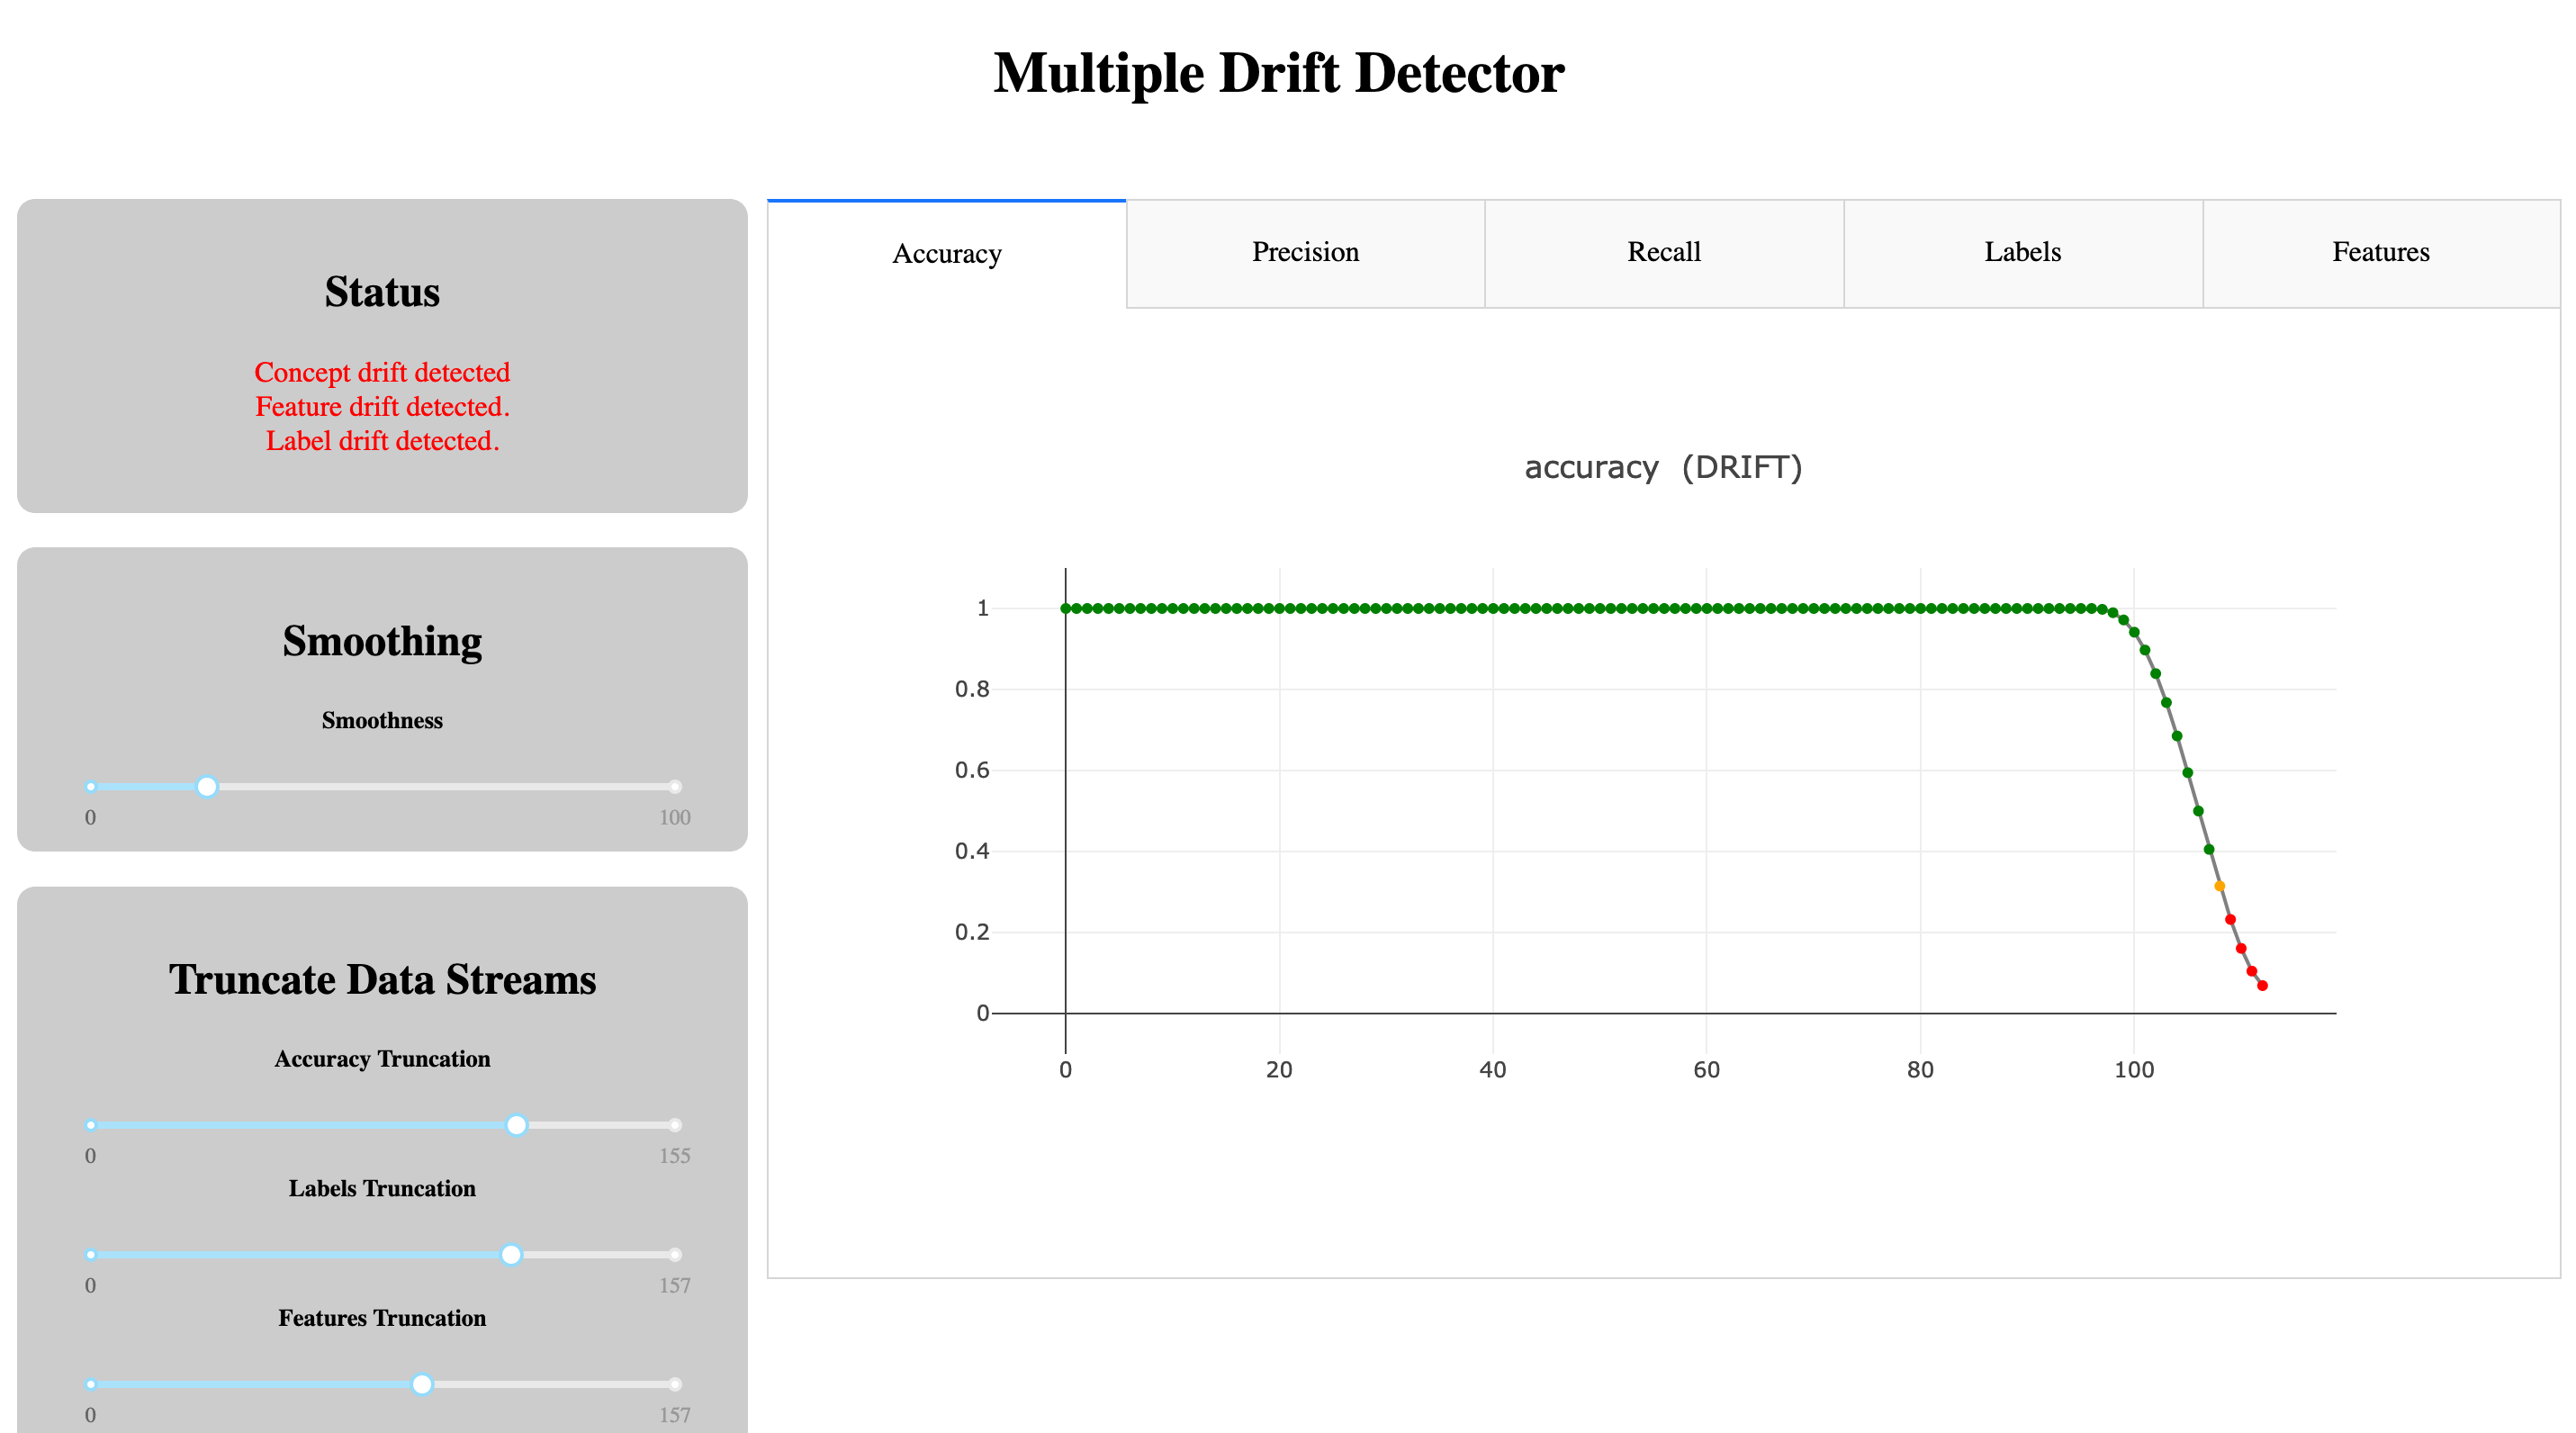
\includegraphics[width=\columnwidth]{images/dash_app.png}
    \caption{The graphical interface for multiple drift detector.}
    \label{fig:dash_app}
\end{figure}

%-------------------------------------------------------------------
% ILLUSTRATION
%-------------------------------------------------------------------

\section{Illustration} \label{mdd:illustration}

In this scenario we illustrate the multiple drift detectors framework using our GP referrals triage motivating example. We explore three drift scenarios, and describe how multiple drift detector will facilitate responding to the drift appropriately. 

\subsection{Scenario 1: Retrain}

Data scientists get a message from the multiple drift detector saying that model recall has decreased for priority 4, and precision has decreased for priority 3, as shown in Figure \ref{fig:scenario1}. Upon investigation, it turns out that a new study has come out that says that coronavirus is more dangerous than previously thought. Patients with this condition are now given priority 4 rather than priority 3.
Data scientists therefore retrain the model on data since the study came out, and the model is once again up to date.

\begin{figure}
    \centering
    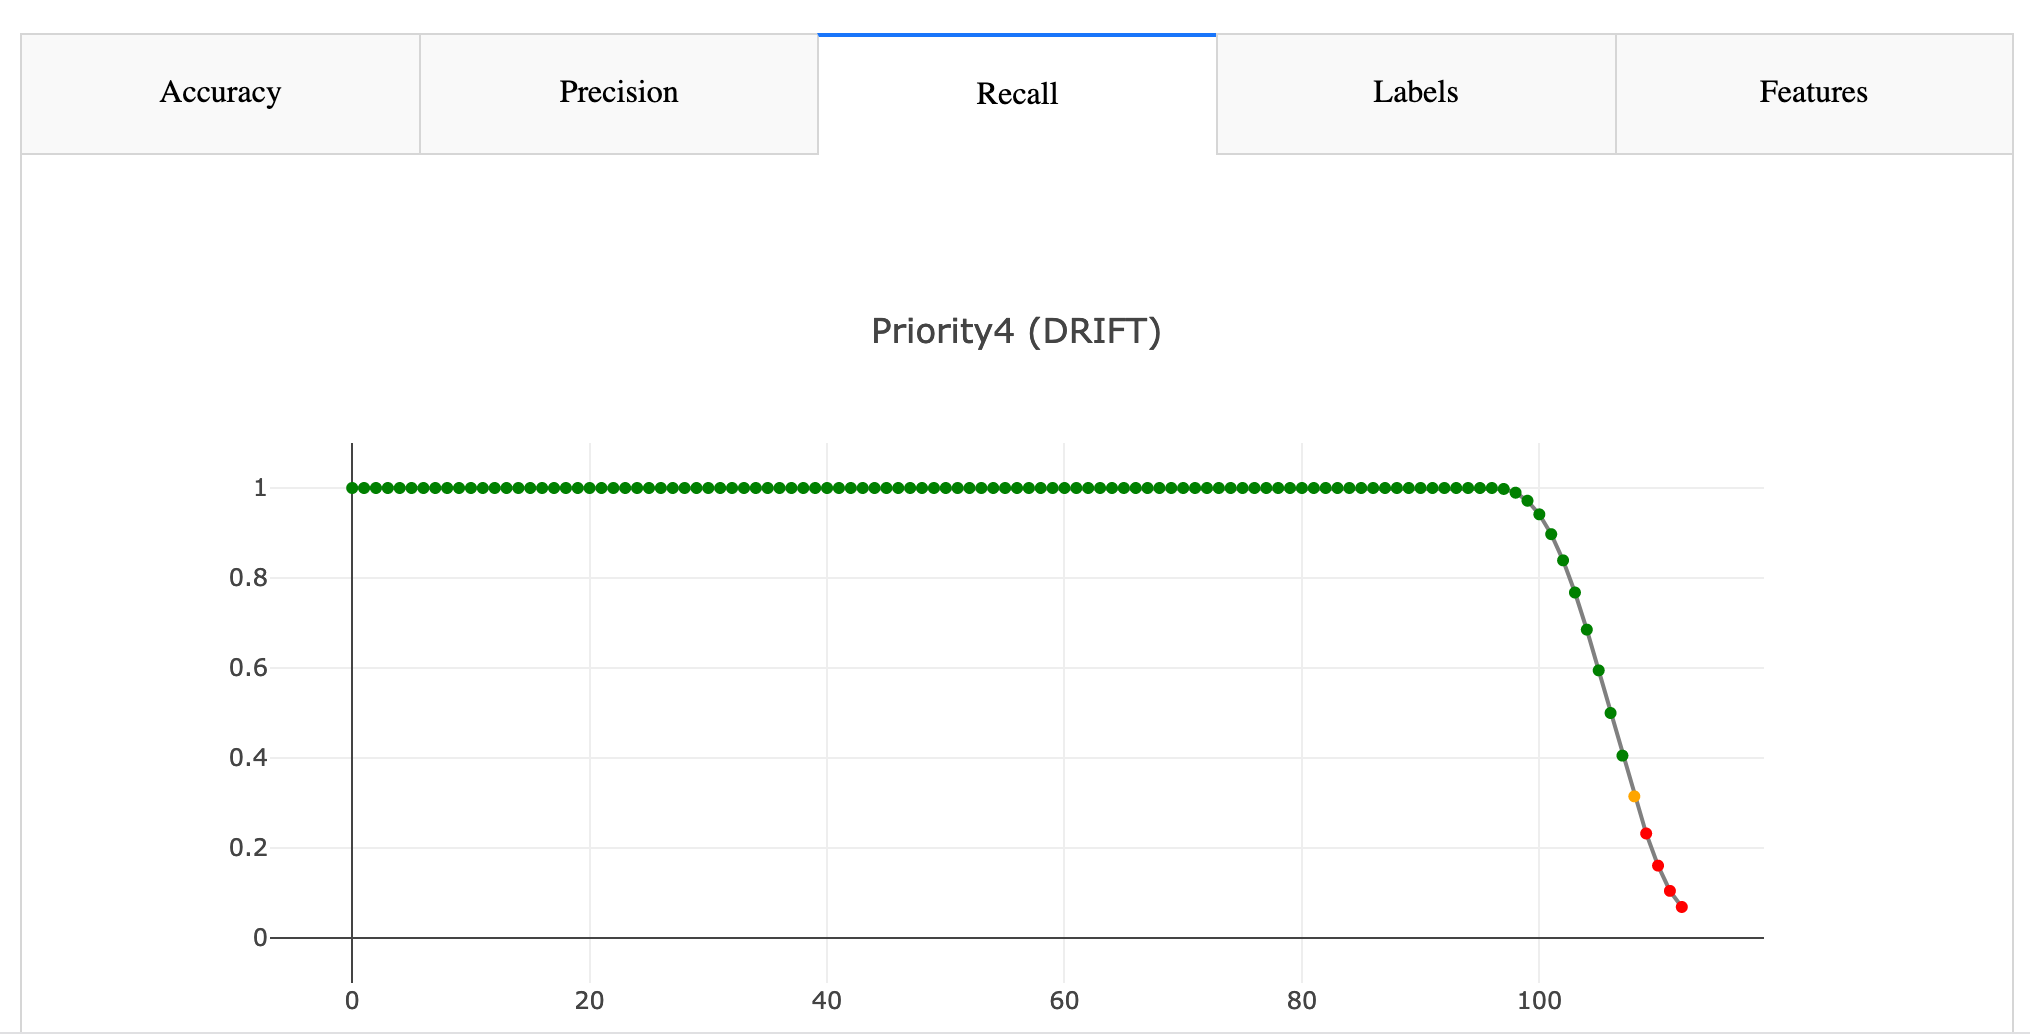
\includegraphics[width=\textwidth]{images/recall_p4.png}
    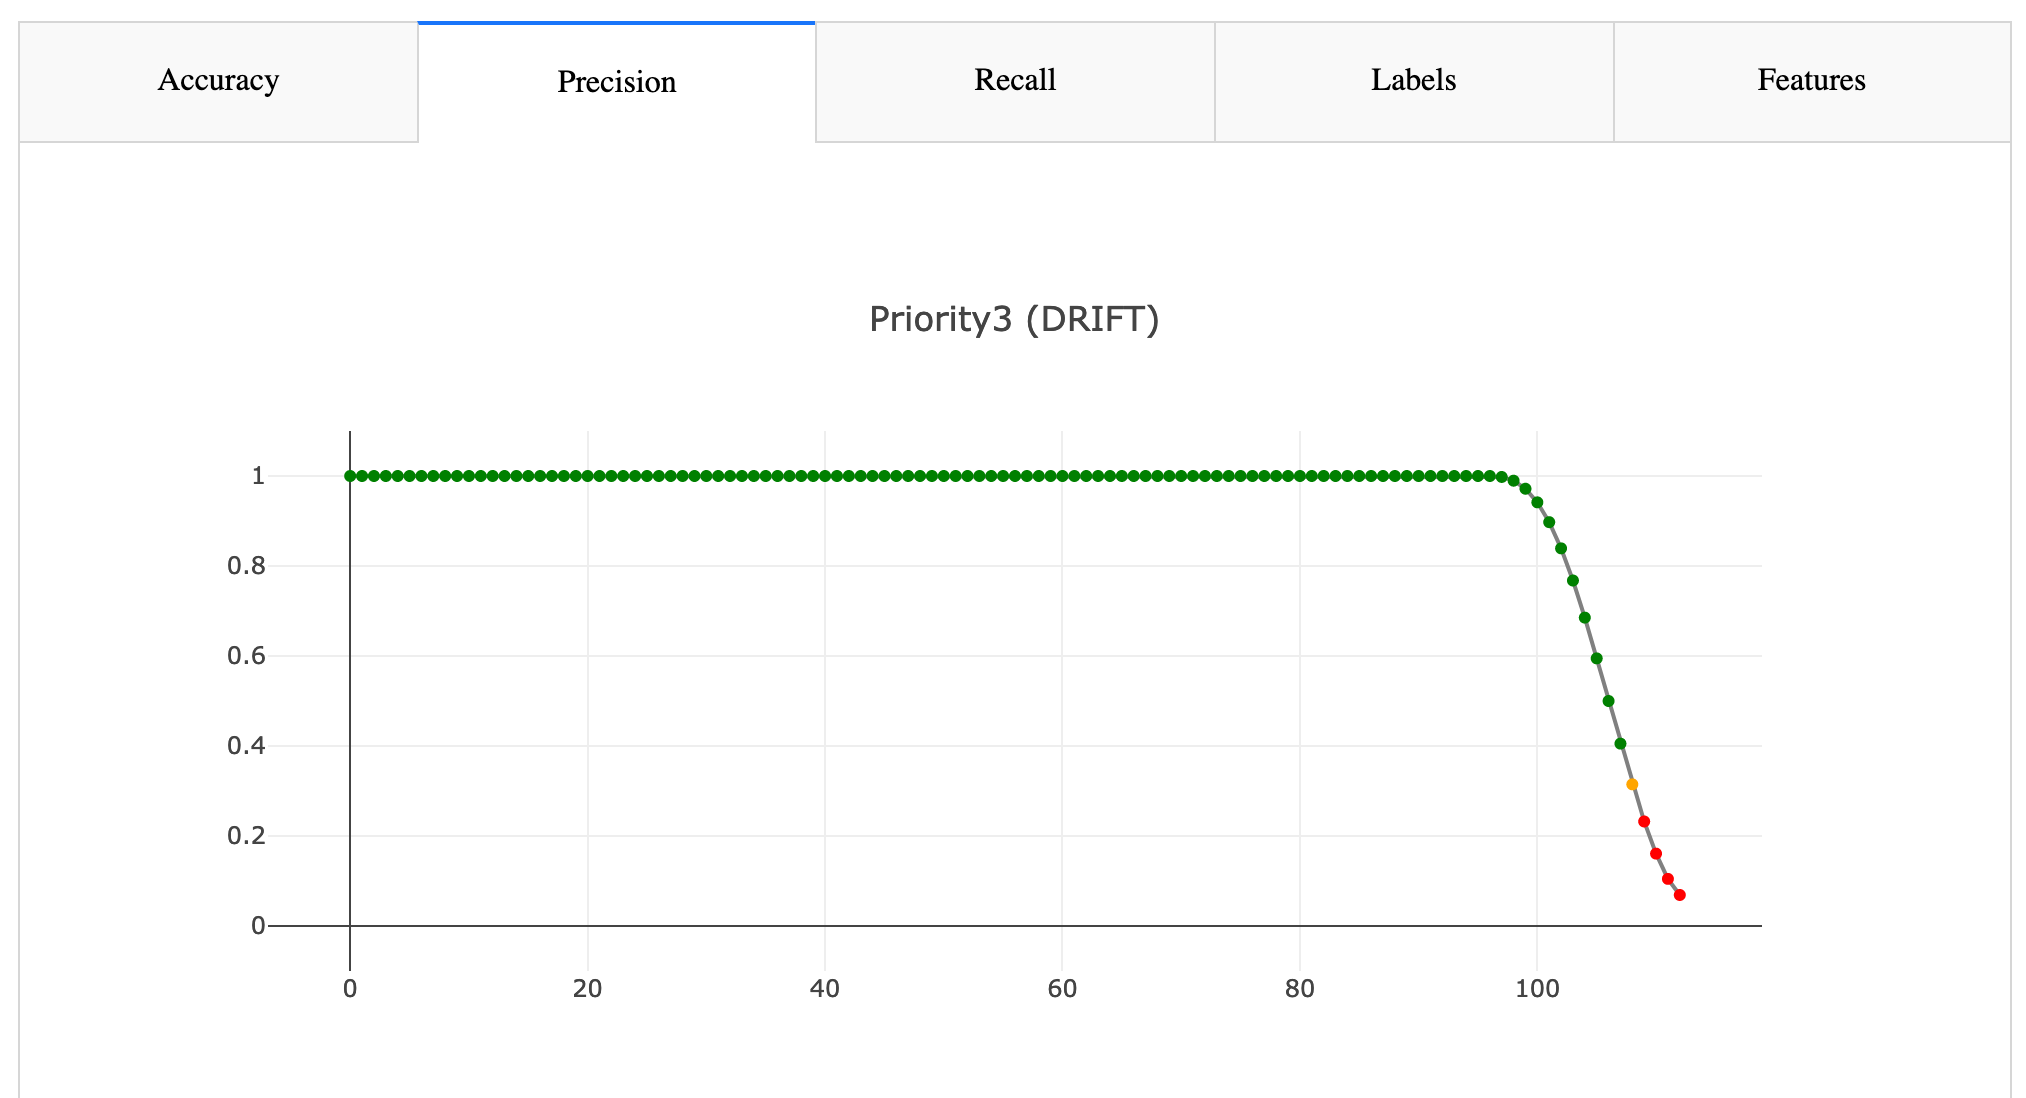
\includegraphics[width=\textwidth]{images/precision_p3.png}
    \caption{Scenario 1: Declining precision for triage priority 3 and declining recall for triage priority 4.}
    \label{fig:scenario1}
\end{figure}
 

\subsection{Scenario 2: No Action}

Data scientists get a message saying that feature drift and label drift have both occurred. Looking closer at the feature drift, it appears that there has been an increase in referrals for patients with coronavirus. Because these instances are given priority 4, there has also been an increase in priority 4 labels, hence the label drift. See Figure \ref{fig:scenario2}. The data scientists decide that this is probably correct behaviour, and the model has seen coronavirus referrals before so this is an instance of on-manifold feature drift. 
The data scientists keep an eye on the model to make sure this plays out as expected. Indeed, the performance metrics don't change significantly. Thus no action is taken.

\begin{figure}
    \centering
    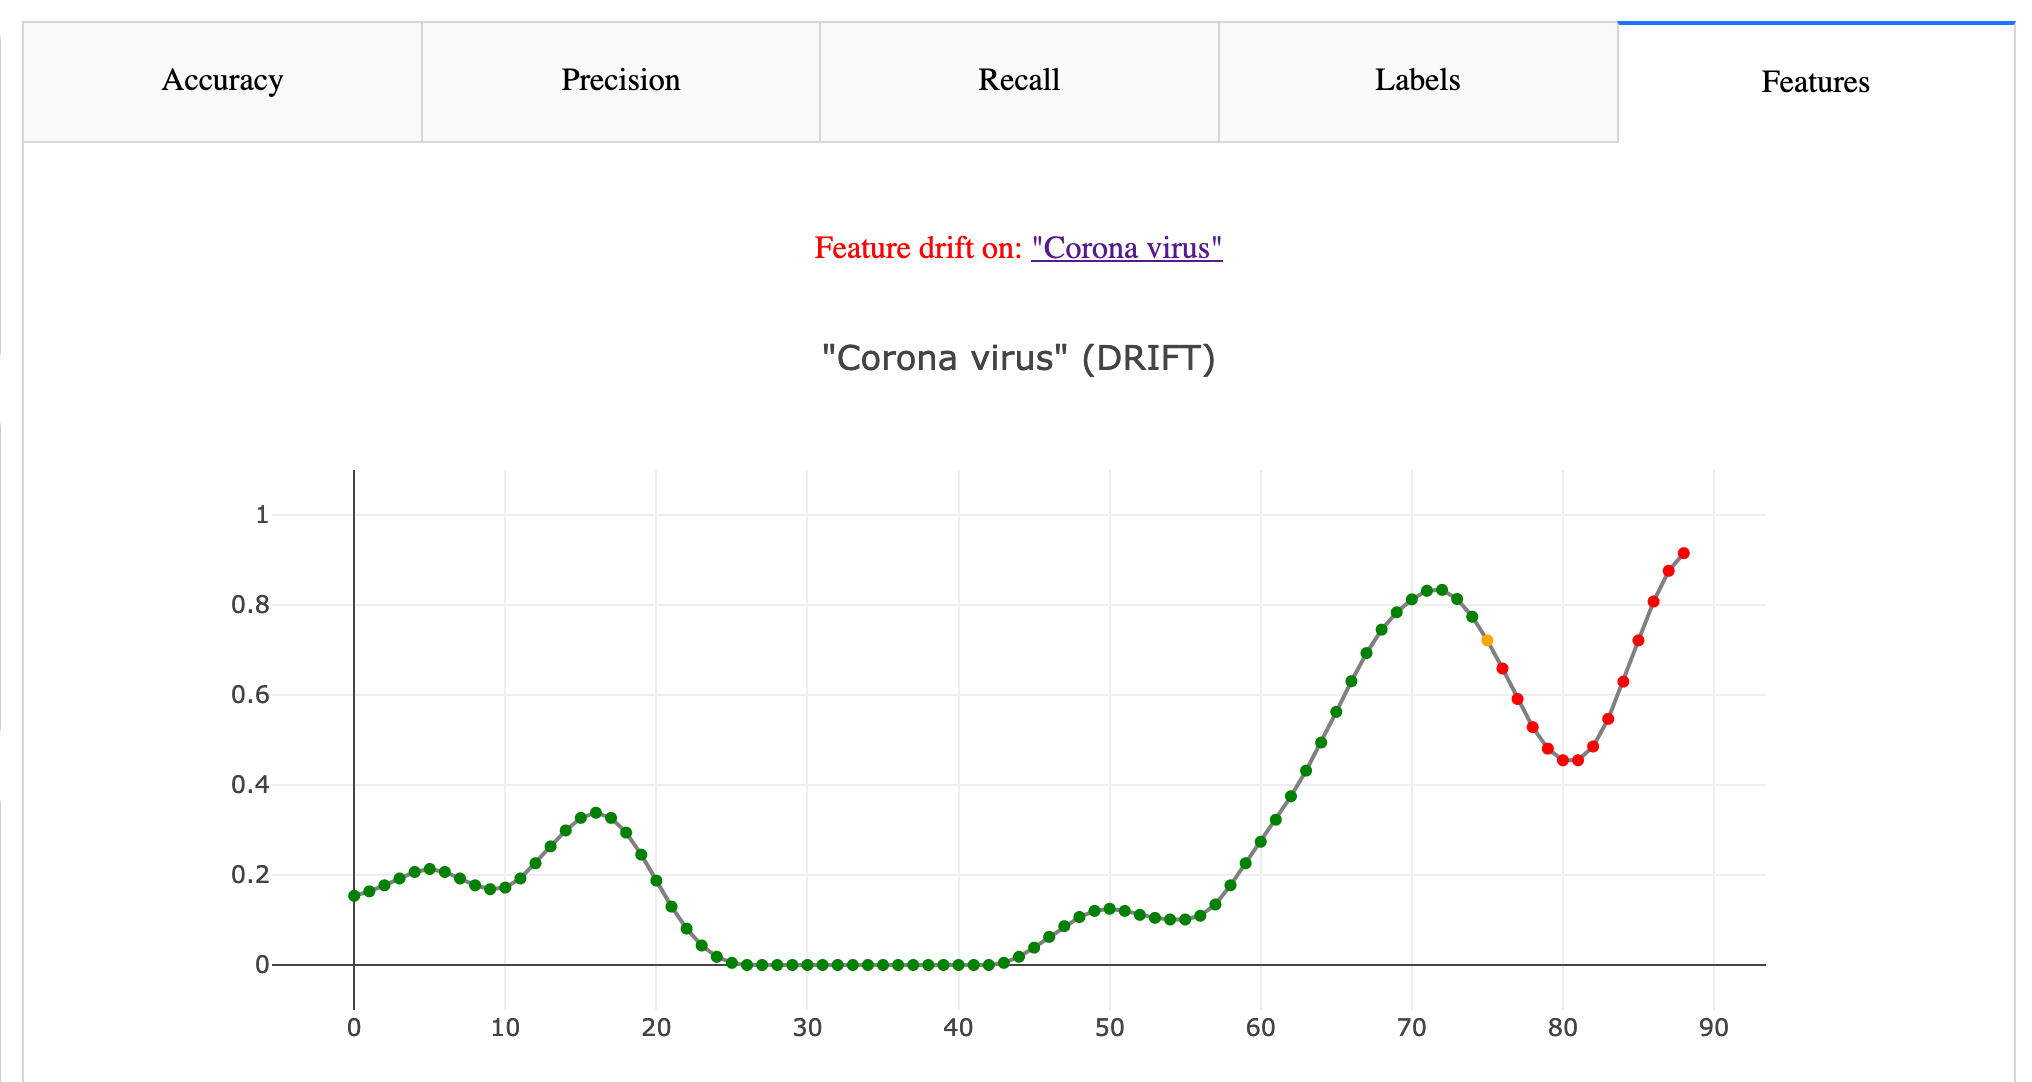
\includegraphics[width=\textwidth]{images/corona_virus.png}
    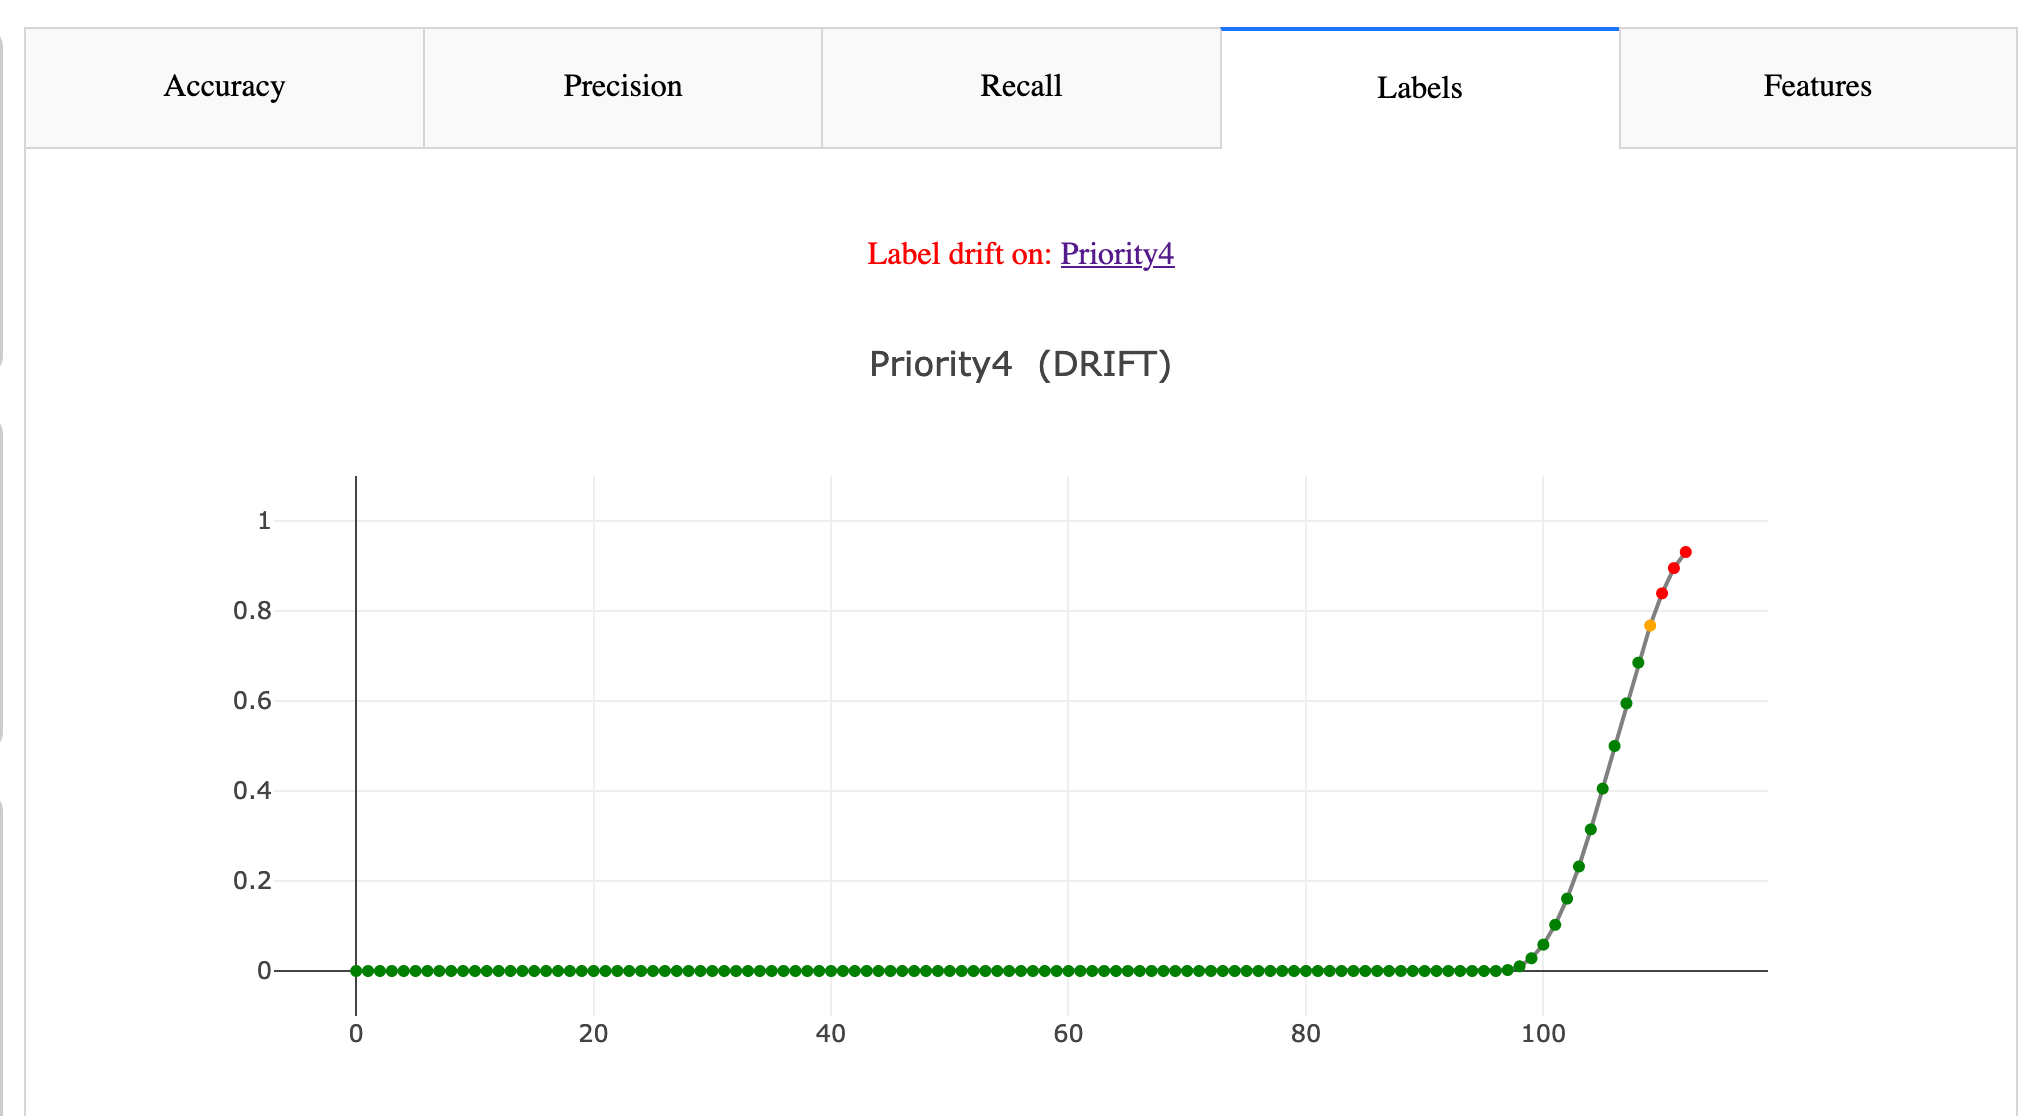
\includegraphics[width=\textwidth]{images/priority4.png}
    \caption{Scenario 2: Increase in the rate of triage priority 4 and increase in the rate of feature ``Corona virus".}
    \label{fig:scenario2}
\end{figure}


\subsection{Scenario 3: Recall}

Data scientists get a message saying that feature drift has occurred. 
Looking closer at the feature drift, it appears that there has been an increase in referrals for patients with coronavirus, as shown in Figure \ref{fig:scenario3}.
Because there were no coronavirus patients in the training data, the data scientists conclude that the model will be unable to make sensible triage predictions for this current wave of patients.
These predictions are therefore clinically unsafe, and so should be withdrawn from the decision support system.
They therefore add a business rule to the priority prediction module stating that if a patient has coronavirus, the model should refrain from making a prediction, and annotate the referral as requiring a clinician to label it.
Once a sufficient dataset of labels for coronavirus patients has accumulated, the model is retrained to handle this new class of patient referral. 

\begin{figure}
    \centering
    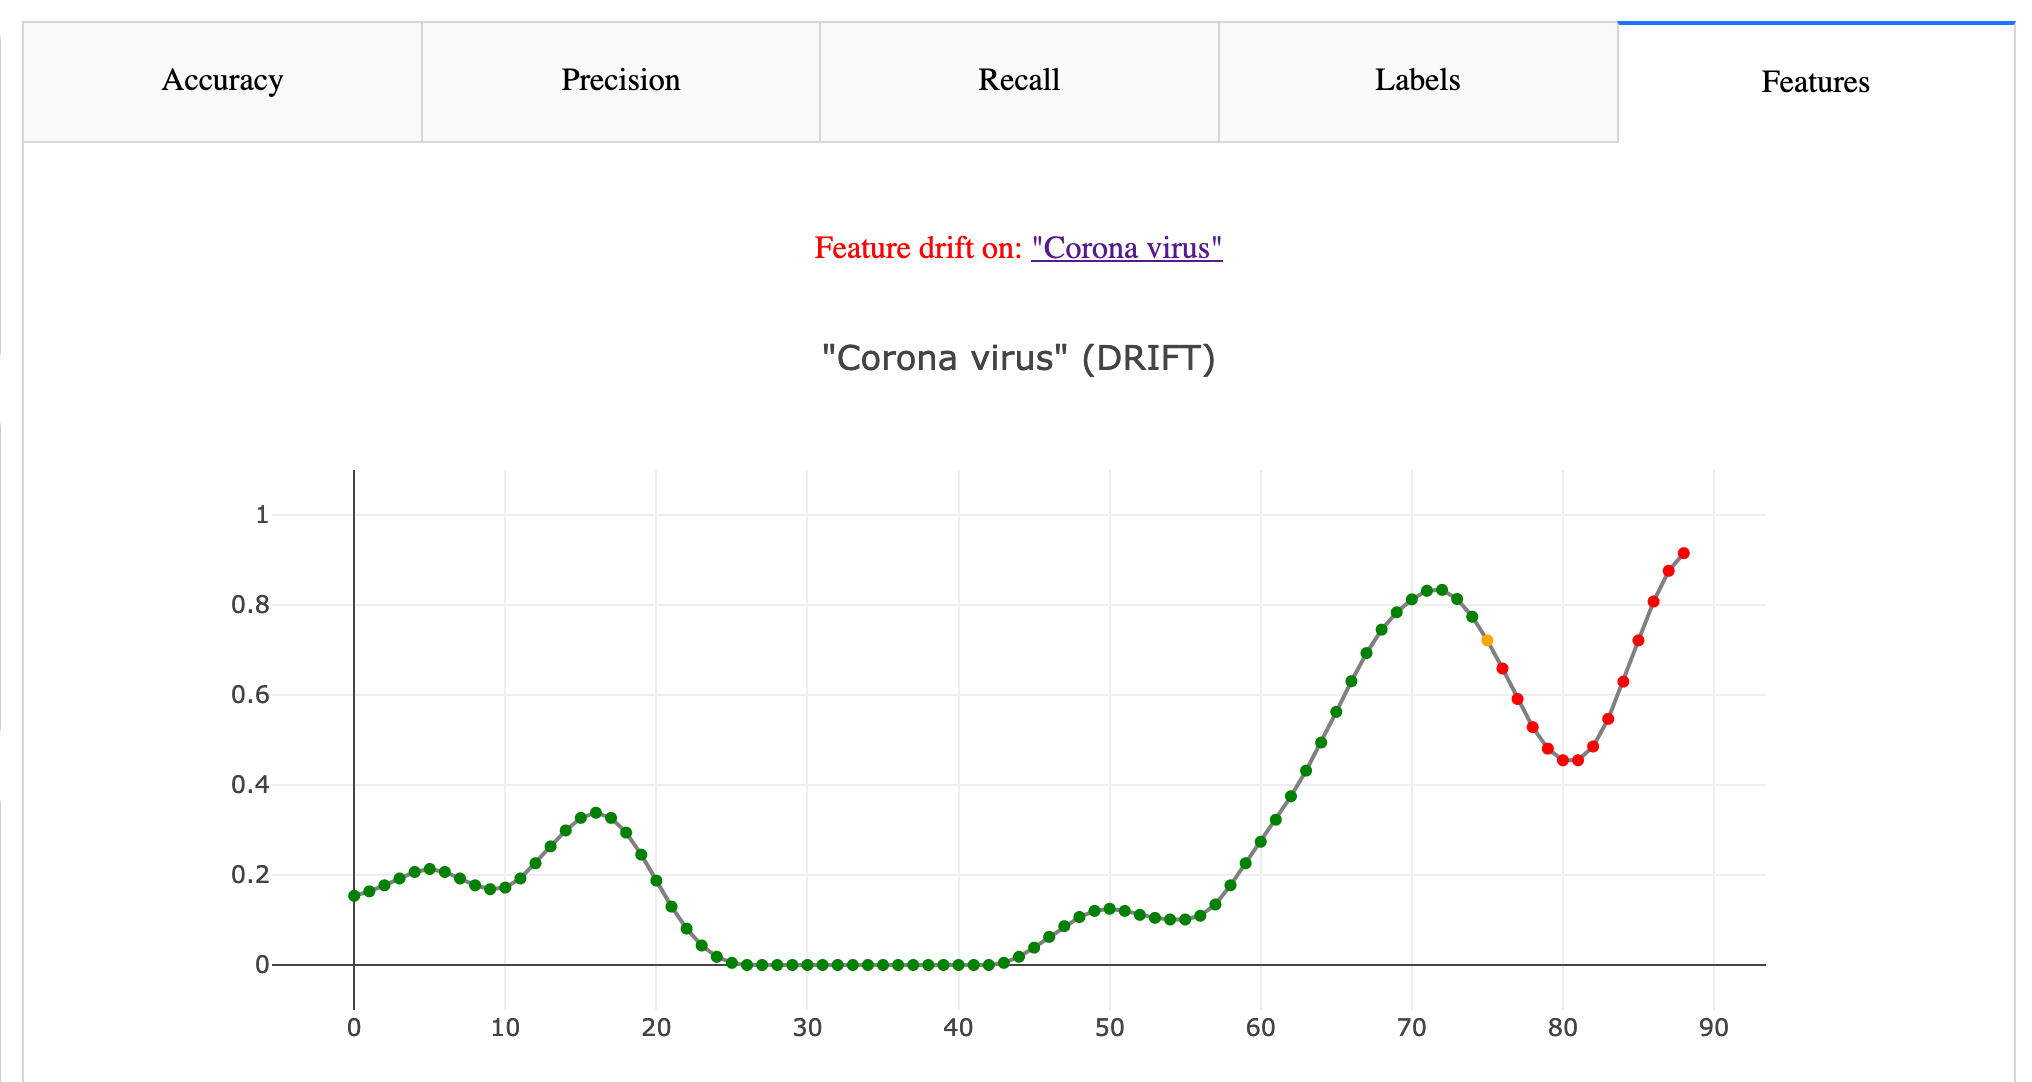
\includegraphics[width=\textwidth]{images/corona_virus.png}
    \caption{Scenario 3: Increase in the rate of feature ``Coronavirus" only.}
    \label{fig:scenario3}
\end{figure}


%-------------------------------------------------------------------
% CONCLUSION
%-------------------------------------------------------------------

\section{Conclusion} \label{mdd:conclusion}

In this chapter we ask ``are existing approaches to concept drift detection suitable for practical data science, and if not how can they be modified to become so?" We argue that there are many implicit or explicit ``axioms" of concept drift detection which will not obtain in practical data science. In particular, we use GP referrals triage as a motivating example for this discussion. We argue for a new operationalisation of concept drift, which we suggest is better suited for practical data science in general, and GP referrals triage in particular. We call an implementation of this operationalisation a multiple drift detector, and explain how to construct such an entity from existing drift detection methods. We also present a graphical interface for a multiple drift detector. We then return to our motivating example of GP referrals triage, and discuss three scenarios in which multiple drift detector would be valuable.
